\documentclass[legalpaper]{article}
\title{\vspace{-4cm}CS3104 Practical Week 1}
\author{170025298}
\date{}

\usepackage{graphicx}
\usepackage[utf8]{inputenc}
\usepackage[font = {small,it}]{caption}
\graphicspath{{images/}}

\usepackage[margin=1.2in]{geometry}

\pagenumbering{arabic}

\begin{document}
	\maketitle
	\section{Design}
	The program will reserve a large memory space for storing things including meta-data, which is a linked list and the data that user required. Users will get a starting address and a free memory space of required size during their using.
	\begin{figure}[h!]
	\centering
	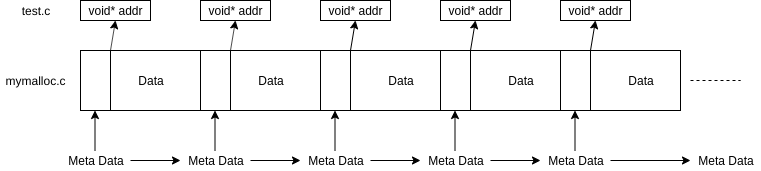
\includegraphics[width = \textwidth]{P1}
	\caption{Basic design}
	\end{figure}
	\subsection{Dynamic Allocation}
	Dynamic memory allocation needs users call the memory allocating functions in case of reserve memory space for arrays or structures. The memory space will contains an invisible linked list and a visible data area.
	\subsection{Memory Reservation}
	A large memory space will be reserved for storing all compulsory things that needed by dynamic memory allocation. Such memory space will be used and might be able to increment during the implementation.
	\subsection{Meta-data and free list}
	Meta-data is a structure of data blocks and three elements will be stored inside: \textbf{size, next and free}.\\
	\textbf{Size} is the size of the data block, which will be used for calculating the distance between blocks. Size can be used to find specific data with several arithmetic on address; \textbf{Next} will store the address of the next meta-data block, which can be regarded as a linked list for storing the using and not used data block as a free list. This will be convenient for freeing node and quickly find the required node. \textbf{Free} is just a status showing whether the block is being freed. Free will be set to IS\textunderscore USE during malloc and set to IS\textunderscore FREE after free.
	\begin{figure}[h!]
	\centering
	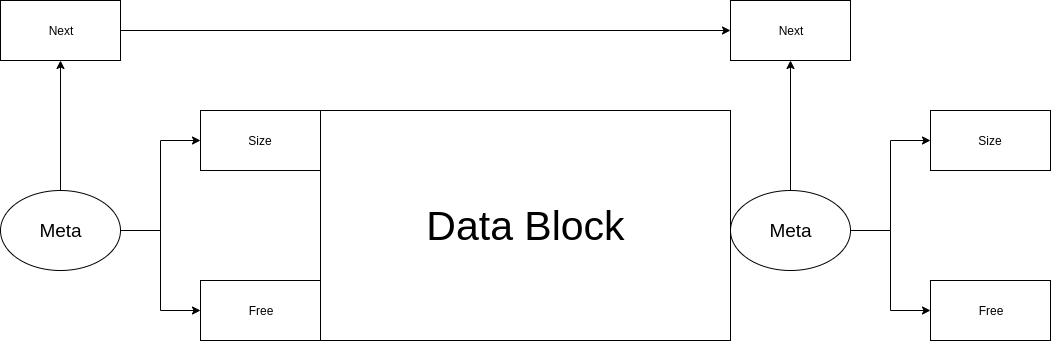
\includegraphics[width = \textwidth]{P2}
	\caption{Data block}
	\vspace{7mm}
	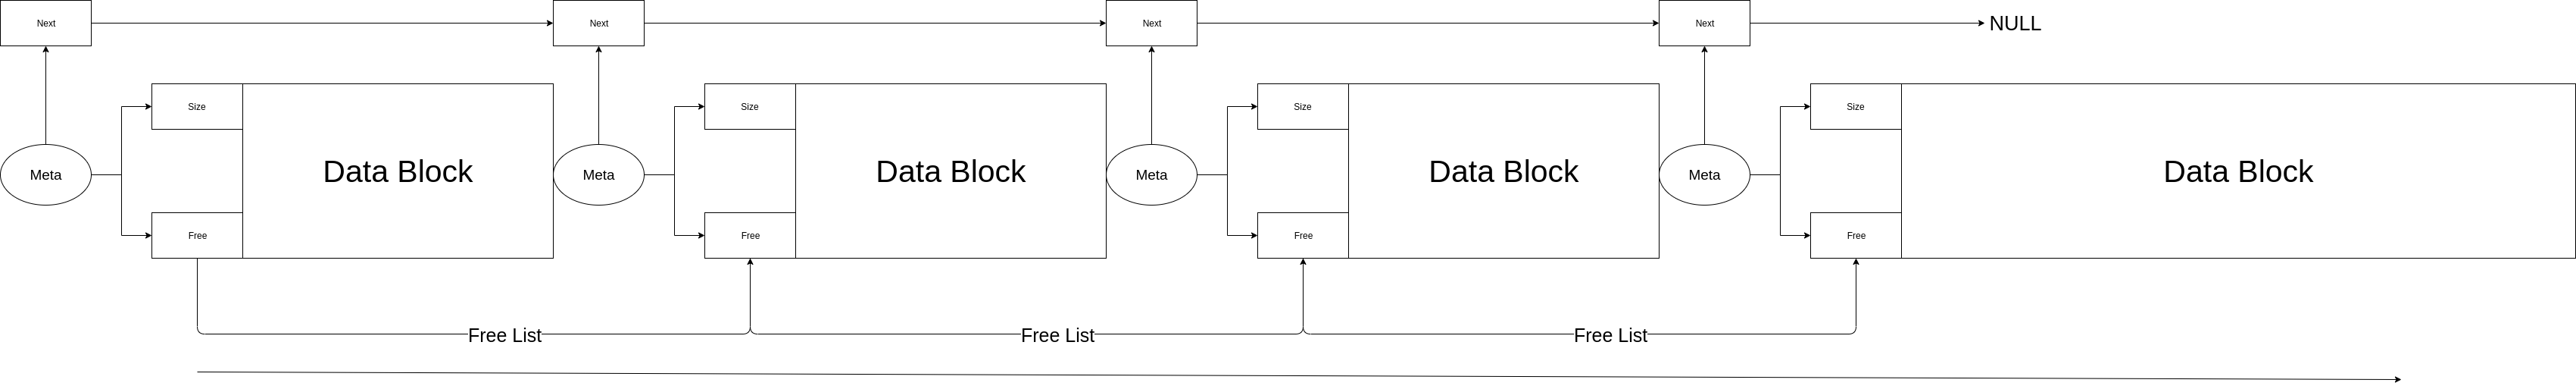
\includegraphics[width = \textwidth]{P3}
	\caption{Memory visualisation}
	\end{figure}
	\subsection{Return Address}
	Memory allocation and freeing are based on operations and arithmetic calculations on addressing pointer. Users will get a pointer which points to the starting address after the meta-data block. 	
	\section{Implementation}
	\subsection{Pages Allocation}
	Pages are allocated by mmap() and keep it private and anonymous and its space are not incremented during basic programming, but may increment during extension. 25 megabytes are allocated to suit all testing on stacscheck.
	\subsection{Header block}
	Header blocks are programmed with struct type and one initial header are setted as global variable as the initial header for the free list. Initial header will be kept NULL until first myalloc functions are to be called by users.
	\subsection{Memory Allocation}
	When Users calls myalloc(), the free list will be created for the first time while such function are being called.
	\subsection{Free List}
	\subsection{Free Space} 	

	
	\section{Testing}
	
	\section{Summary}
	
	\section{Extensions}
\end{document}